\section{Overall Description}
\label{sec:overall_description}
This section is intended to provide an overall description of the WOMS product, its users and business environment, and lastly the assumptions made for this project as well as present the applying constraints.
\subsection{Product Overview}
The project in hand will be a WOMS, Work Order Management System.  The purpose of this system will be to handle work orders, for maintenance, repair and construction procedures. The system will dispatch work orders to the appropriate field technician, depending on the technicians location and competence. The system will also have capability to prioritize  work orders  making the currently  most important work executed first. WOMS will also support the field technicians in their work process as they may through a WO access information related to maintenance work, such as manuals and system equipment specifications. 

The above mentioned functionality concerns the pre- and the main phase of maintenance work (create, dispatch, and execute WOs). The scope of WOMS is also extended to the aftermath and post-phase of maintenance work, for example follow-up work and analysis. The WOMS gather information such as time and material consumed on WOs, information which is the output from FTs. It will also interact with the finance function of ACME, to automatically enter cost reports and other expenditures. 

Let us shift the focus to another division of ACME; as mentioned in section \ref{sec:introduction}, the customer care function is one major cost - fortunately WOMS offers improved utilities to CC. The system will act as real-time status provider over maintenance/repair/construction work, in other words: providing always up-to-date outage information. 

\subsection{Product Stakeholders and Users}
\label{sec:produt_stakeholders_and_users}
The product stakeholders have been identified and categorized in a Stakeholder Categorization, see appendix \ref{appendix_b_stakeholder_categorization} to view the model. Furthermore, an Actor Table describing the users, their roles and responsibilities in the system context, can be found in table \ref{table:actor_table}. As one can see, the table shows the different roles direct users (internal and external stakeholders) enact when interacting with the system, and also what actor roles current systems will have.
\begin{center}
	\begin{longtable}{|l|p{7cm}|p{3cm}|}
		\caption{Actor table}
		\label{table:actor_table}\\
		\hline
		\textbf{Actor} & \textbf{Attributes and Responsibilites} & \textbf{Job Title(s)}\\
		\hline
		\endfirsthead

		\multicolumn{3}{c}%
		{\tablename\ \thetable\ -- \textit{Continued from previous page}} \\
		\hline
		\textbf{Actor} & \textbf{Attributes and Responsibilites} & \textbf{Job Title(s)}\\
		\hline
		\endhead

		\hline \multicolumn{3}{r}{\textit{Continued on next page}} \\
		\endfoot
		\hline
		\endlastfoot
		\hline
		Equipment informer& Supply WOMS with system and equipment information, e.g. manuals, parts & NIS \\
		\hline		
		Work Order Creator&Responsible for creating work orders WOMS shall handle &M/E, MO, CC  \\
		\hline
		Service controller&Interact with the system to get status information for a maintenance/repair service. This will tell the status for an outage 
		&M/E, MO, CC, CIS \\
		\hline
		The ''Wallet''&When WOMS order a service, it is this actor's responsibility to approve or deny the requested service. Must also receive and store incoming cost reports &ERP (PU) \\
		\hline
		Maintenance executor&Responsible for executing the dispatched work orders from WOMS. Update the status for a work order and report time and material used when a job is done &FT \\
		\hline
		Dispatcher&To select the most appropriate field technician to be assigned a work order and consequently dispatch it  & M/E, MO\\
		\hline
		Analyzer&Analyze cost and repair time data retrieved from WOMS to improve cost and work processes &ACC \\
		\hline
	\end{longtable}
\end{center}

\subsection{Product Environment}
\label{sec:product_environment}
This section with subsection 2.3.1-2.3.6 describes all the business processes and model them (modeled as \emph{Process Maps} according to White \cite{bpmn}) to illustrate how they are connected to the WOMS specified in this project. In addition, a \emph{Context Diagram} is presented in appendix \ref{appendix_a_context_diagram}, to illustrate the environment with WOMS together with direct users and other systems. 
\subsubsection{Planning Maintenance Work}
\label{sec:bp1}
The maintenance work is a large cost driver for ACME, as stated in section \ref{sec:introduction}, and to be able to fulfill the goal GOAL-1 - maintenance work is one process that needs to be improved and increased in efficiency. The \textbf{Planning Maintenance Work} process seeks to satisfy these needs. 

In this process, the stakeholders M/E together with the ACC are the main players. M/E analyze the different systems and existing equipment to identify maintenance work to do. This includes browsing through information; such as how old a system/equipment is, giving indicators to maintenance needs. If M/E locate such necessity, they project a plan and hand it over to ACC who evaluate the plan and its constituents. ACC may find ways to reduce the costs of the plan, e.g. how spare parts will be bought, and finally decide whether it is valuable and motivated to send the plan as a request to PU - to have them sign it. The whole process is modeled in figure \ref{fig:planning}.

The WOMS shall support this process by offer new data to M/E in their "Analyze" activity, e.g. fail-tendencies for different machineries. It shall also support the "Project a plan" activity in a similar way as it will provide data, e.g. statistics of how much time is spent maintaining certain systems/equipment, materials that is usually needed and so on, to make it easier to project better plans.
\begin{figure}[H]
	\centering
	\setlength\fboxsep{7pt}
	\setlength\fboxrule{0.5pt}
	\fbox{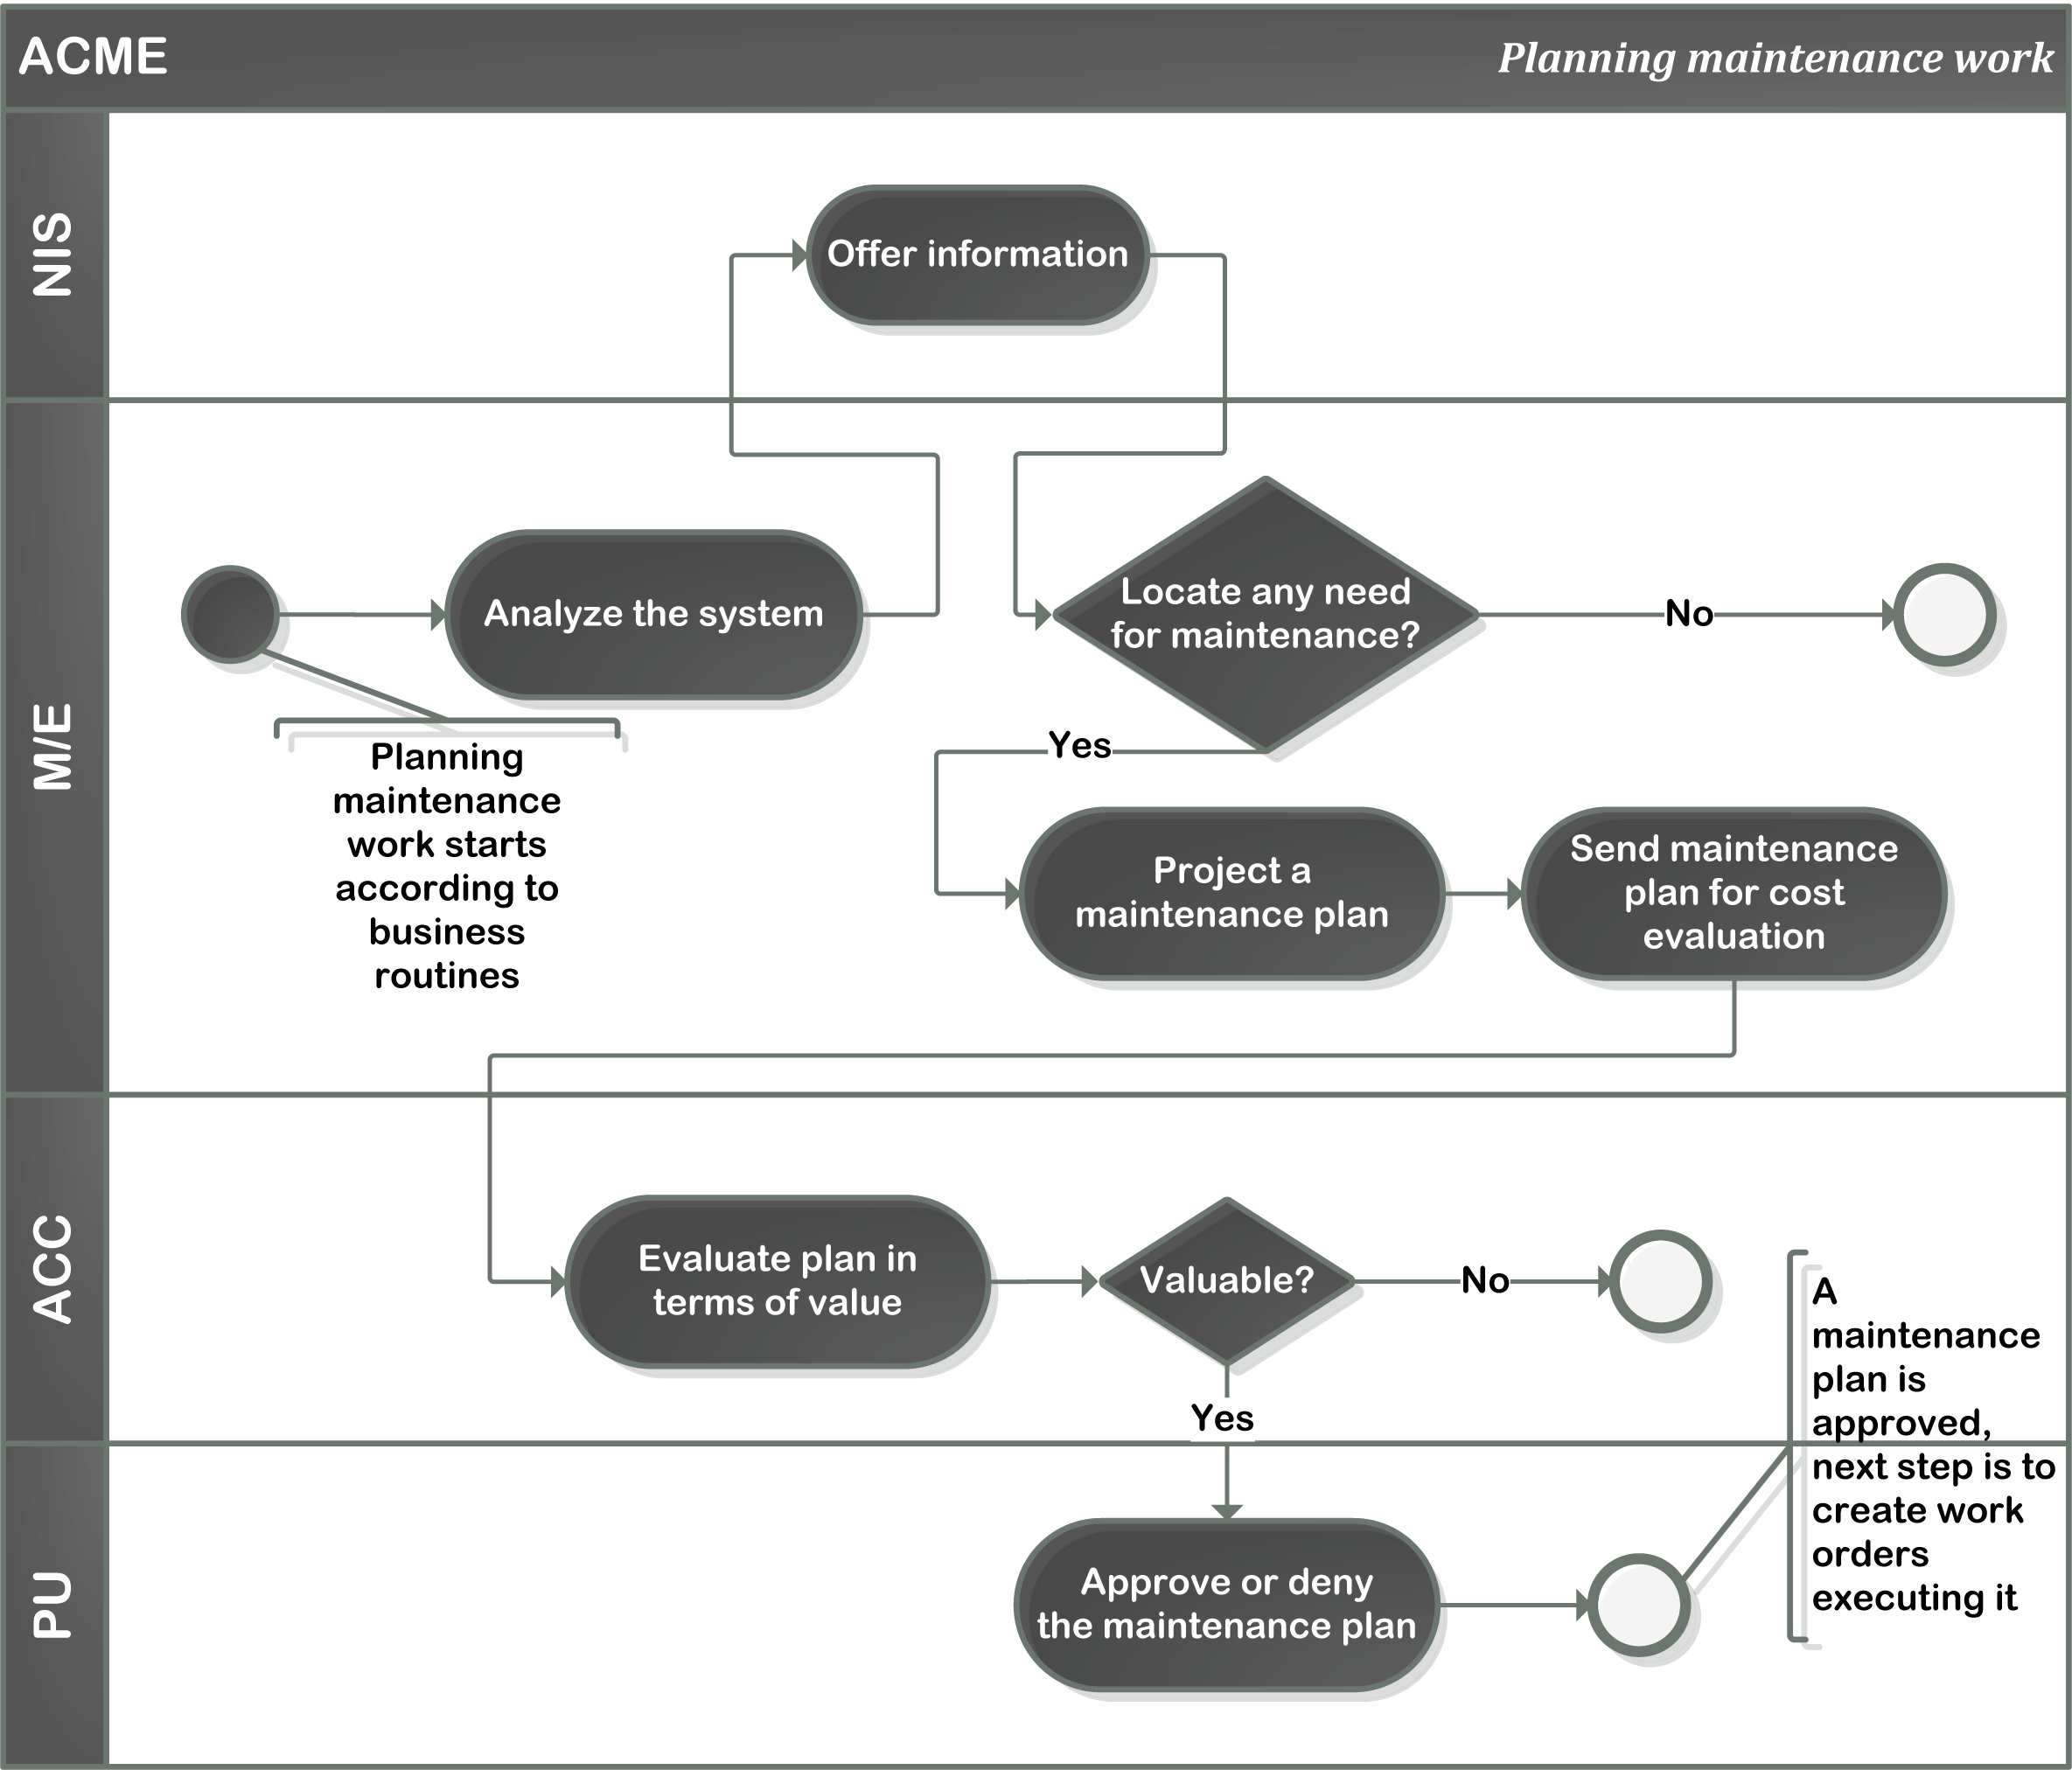
\includegraphics[scale = 0.7]{images/planning.png}}
	\label{fig:planning}
	\caption{Planning maintenance work}
\end{figure}
%
\subsubsection{Creating Work Orders}
\label{sec:bp2}
The \textbf{Creating work orders} process focuses on the way ACME handles work orders. ACME has of today no standardized way of handling work orders. This leads to work orders gets lost and don't get executed even when they were suppose to. In some cases the opposite happens, work orders that the purchasing team think is too expensive gets executed because they were not consulted before the work order was executed. This process that both make it clear for the company how they should handle their work orders is in the biggest of needs. This process will help the achieving GOAL-1, since no unnecessarily expensive work orders will be executed. The process will also help in solving GOAL-2 since no necessary work orders now will be forgotten. 

In this process there are three different main users, MO, M/E and CC. These users have in earlier processes decided that a maintenance/repair/construction work is needed and want to create a work order. This work order then gets automatically updated by the NIS to include all the relevant information about the components and other parts in the planned work order. The work order is then handled by the ERP as a new service where an automatic cost calculation is made. The PU will now read the calculations made by the ERP and they will have the final decision on whether or not to execute the work order, this is not done in the WOMS. The final decision is then delivered to the user specifying it in the first place. The whole process is modeled in figure \ref{fig:create}.

The WOMS is the system where WOs are create and store. The system will also	 help in this process by being a center hub between all the different components in this process. To do this the WOMS needs to be able to transfer data between different systems and have working interfaces for all of these. All the different stakeholders needs to have the an interface that makes it possible for them to create and modify work orders, depending on their work title, which will be stored in the WOMS.
\begin{figure}[H]
	\centering
	\setlength\fboxsep{7pt}
	\setlength\fboxrule{0.5pt}
	\fbox{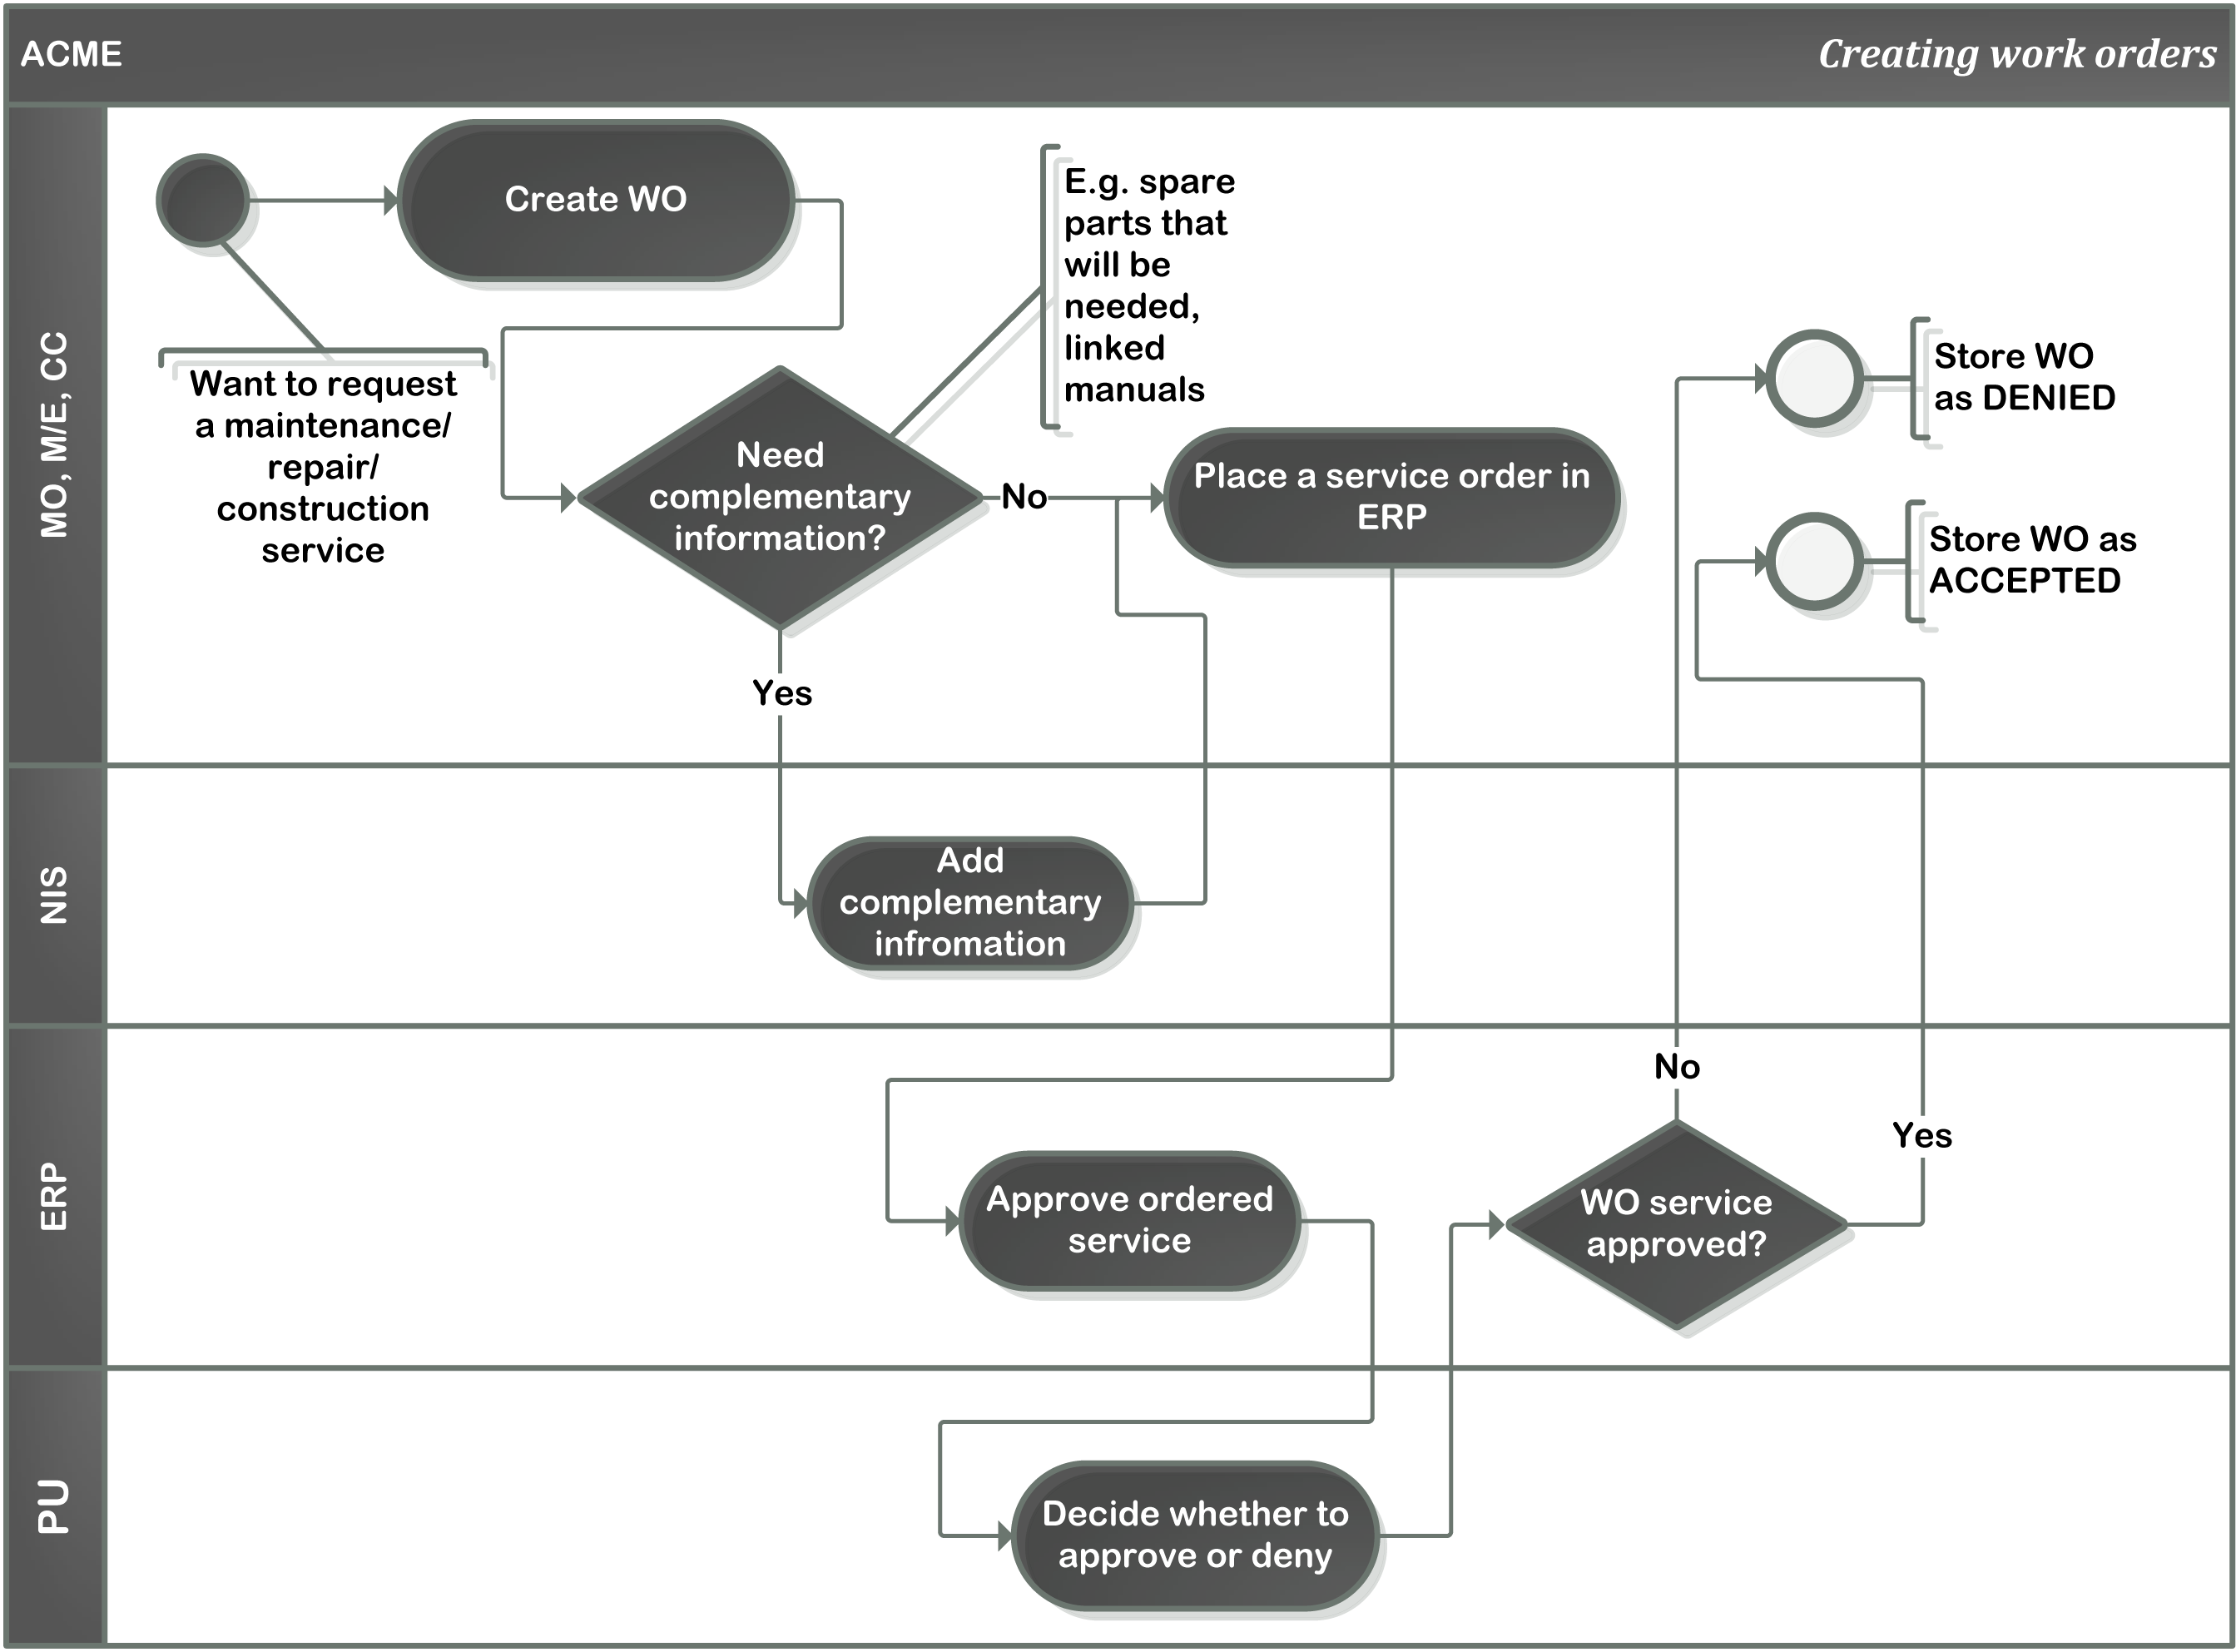
\includegraphics[scale = 0.7]{images/create.png}}
	\label{fig:create}
	\caption{Create work orders}
\end{figure}
%
\subsubsection{Dispatching Maintenance/Repair Work to Technicians}
\label{sec:bp3}
The \textbf{Dispatching maintenance/repair work to technicians} is triggered when there is a created and approved work order, a result from the business process \ref{sec:bp1}. To be able to dispatch work orders in a efficient way will contribute to GOALS-1 and GOALS-2, a reason to this is (for example): when a system or equipment is down (broken), the cost is not only the repair cost itself but also the longer an object is out, the higher the costs will be.

This process begins with - a work order operator (may be M/E or MO) has work orders to dispatch. Information such as the work order's priority, the skills and material needed helps the operator in the process of assigning the work order to a FT. Profiles of field technicians is also available including information such as their geographic position and their competence. Before a work order may be dispatched, the operator sends a request to FT who subsequently responds with accept or deny. If it was accepted, a work order has been dispatched and this business process ends.

WOMS is the underlying system, which enables this process to be executed as recently described. Work order operators works directly with WOMS, viewing WO's and FT's profiles and using the system to interact with FT's. WOMS support the FT's activities as it feeds them with request and work orders, and also receives their responds to requests.
\begin{figure}[H]
	\centering
	\setlength\fboxsep{7pt}
	\setlength\fboxrule{0.5pt}
	\fbox{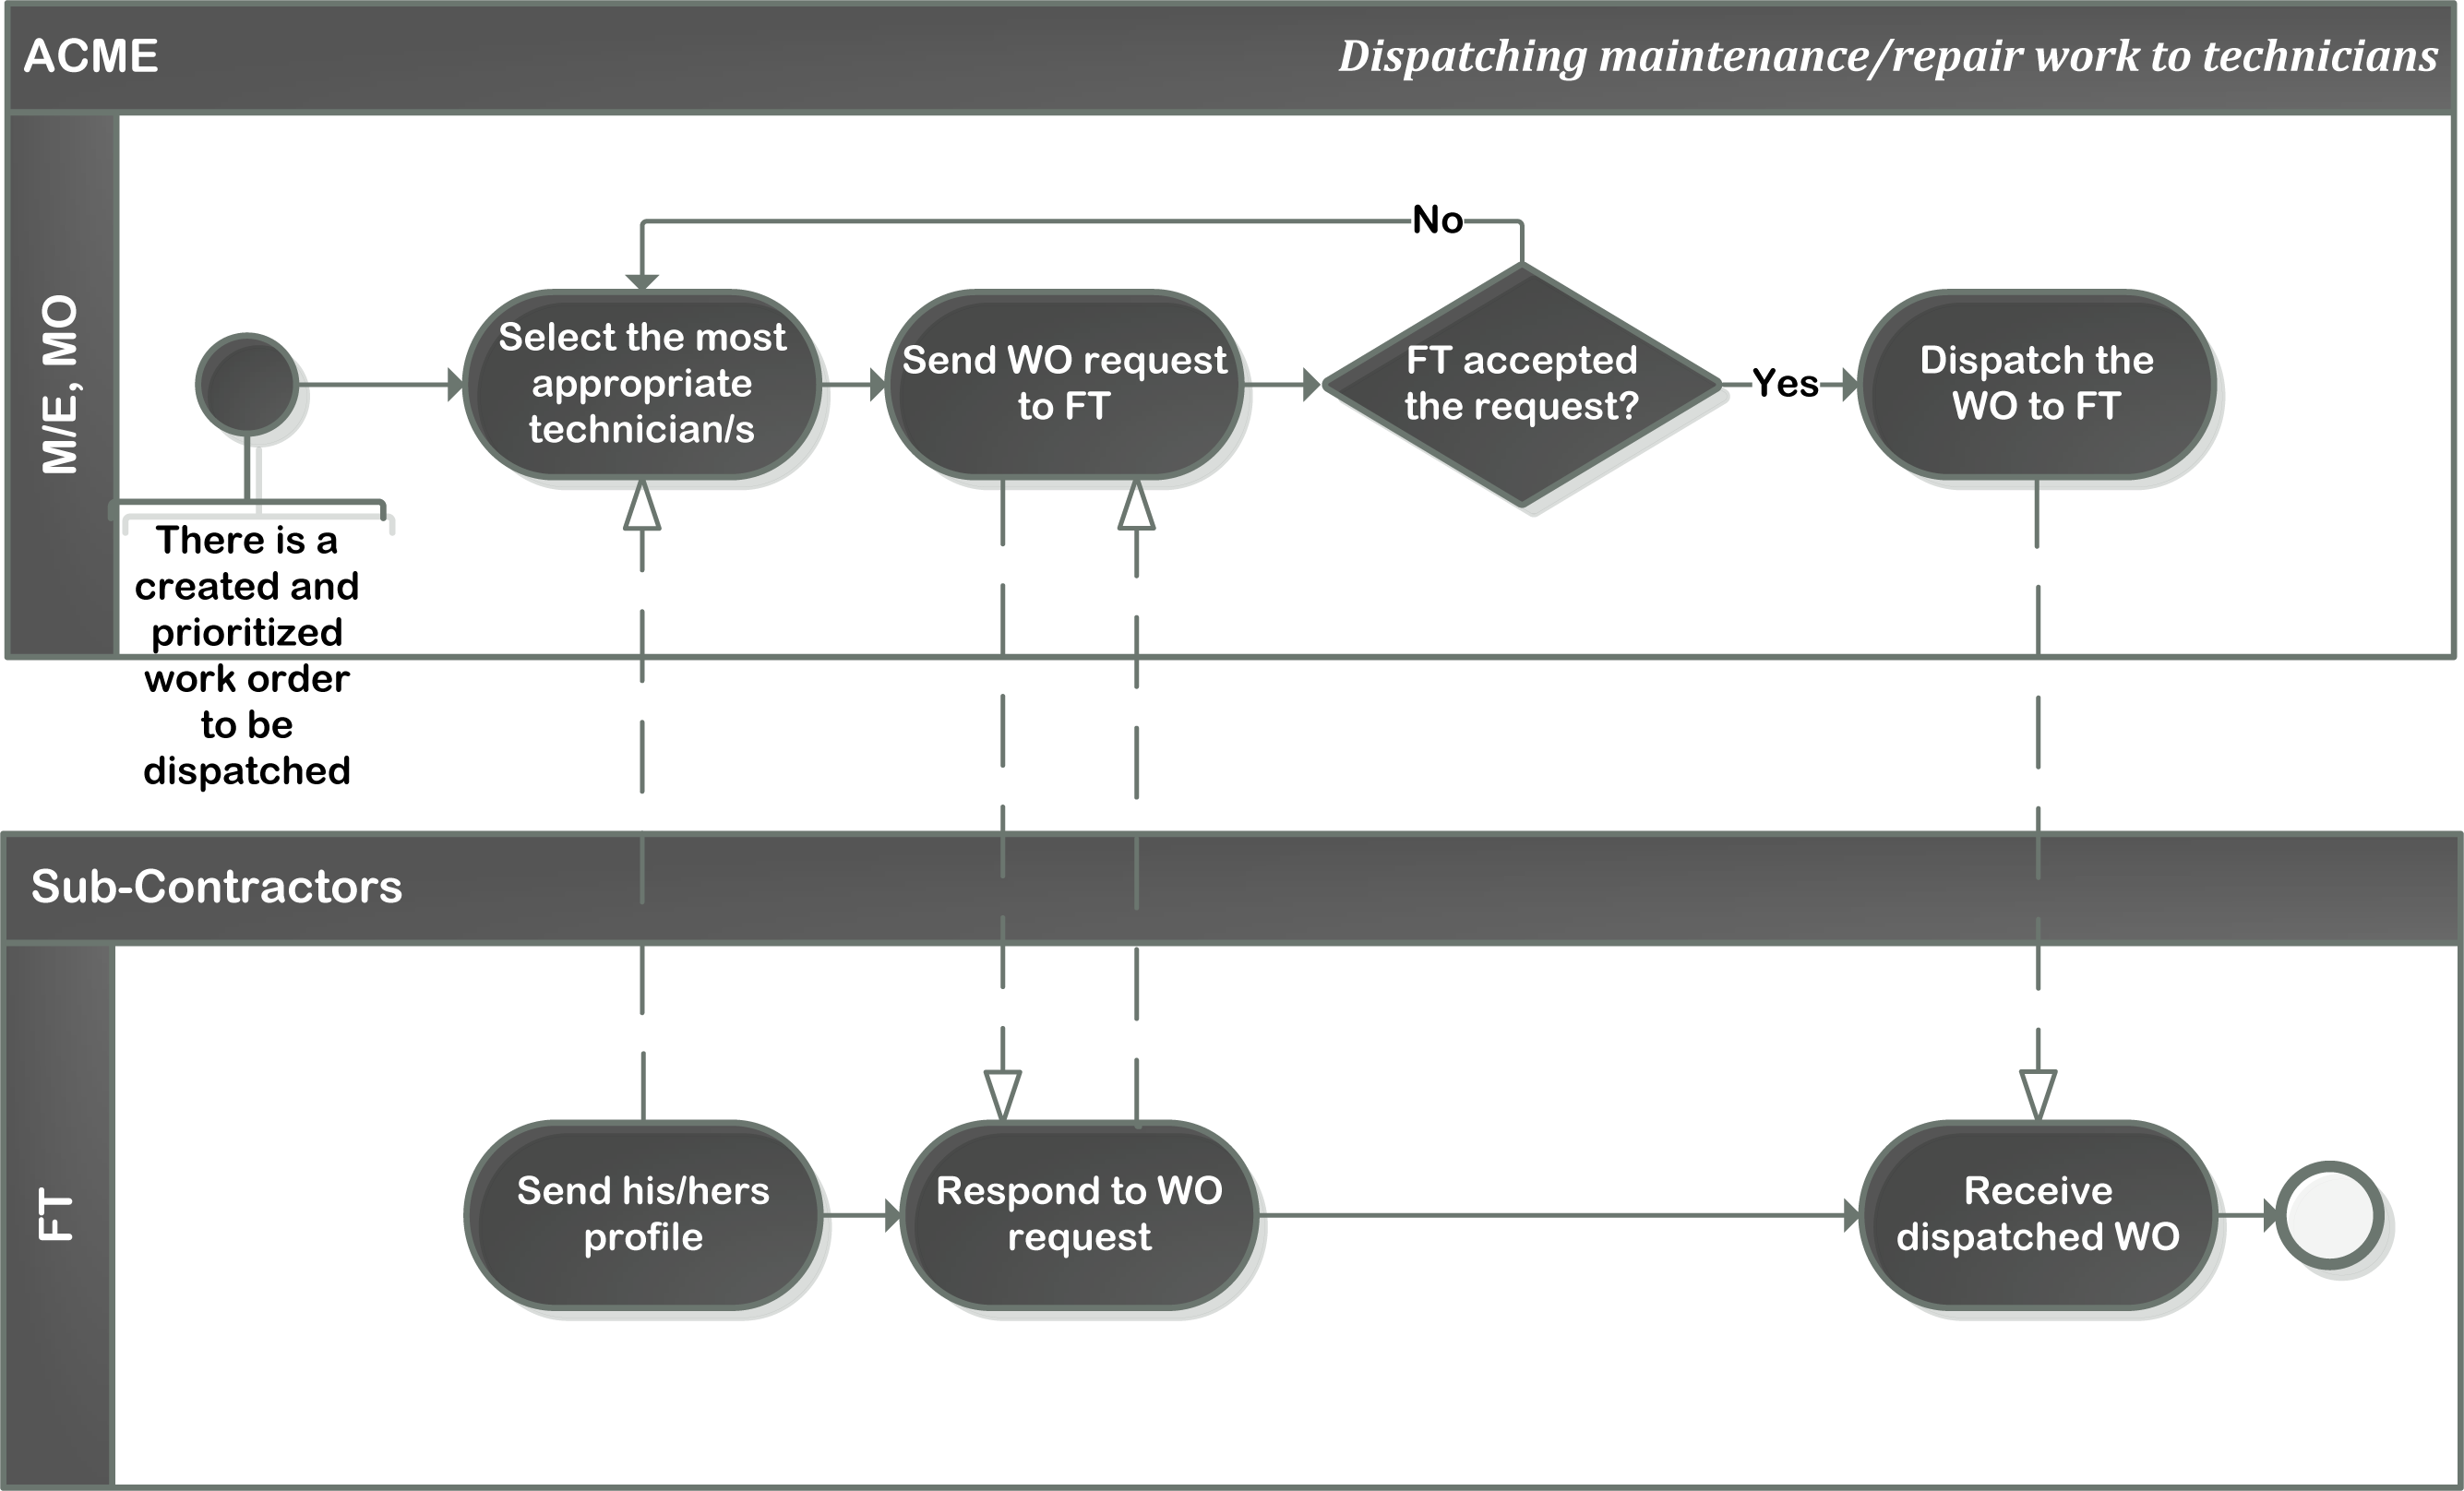
\includegraphics[scale = 0.7]{images/dispatch.png}}
	\label{fig:dispatch}
	\caption{Dispatching maintenance/repair work to technicians}
\end{figure}
%
\subsubsection{Carry Out Maintenance/Repair Work}
\label{sec:bp4}
\textbf{Carry Out Maintenance/Repair Work} affects the business goals GOAL-1, GOAL-2, and GOAL-3. GOALS-1 and GOALS-2 is pretty straightforward connected to this process, as how ACME and FT's carries out and executes work orders directly affects maintenance/repair/construction costs. We will see that costs within the CC division also are \textbf{indirectly} affected.

Figure \ref{fig:carry} shows the start of the process. A FT has been assigned and is about to carry out a WO, thereby FT changes the status of the WO to \emph{ACTIVE}. He or she may also obtain information related to the WO, e.g. manuals. Next step is that FT estimates the time to completion for the current WO and shall also, anytime, during the maintenance work update the estimated time. Having this value to be as correct as possible increases the value of the customer care function (where customer contacts to get answers and information of e.g. an outage) - the more accurate information they have access to, the more satisfied customers will be. At last, when a WO is completed, FT shall report time and material used for the recent work. This information is used in other processes, e.g. \ref{sec:bp1} and \ref{sec:bp6}, and is also subject to a cost report entered in ERP system.

WOMS will support this, first of all since it will be the system that enables the information flow within the process. FT's get the WO itself and its information from WOMS via their PDA. They also, via their PDA, send information to WOMS that stores the information (such as a WO's status, time-material reports). WOMS will also act as the "forwarder" of the cost report, sending it to ERP.
\begin{figure}[H]
	\centering
	\setlength\fboxsep{7pt}
	\setlength\fboxrule{0.5pt}
	\fbox{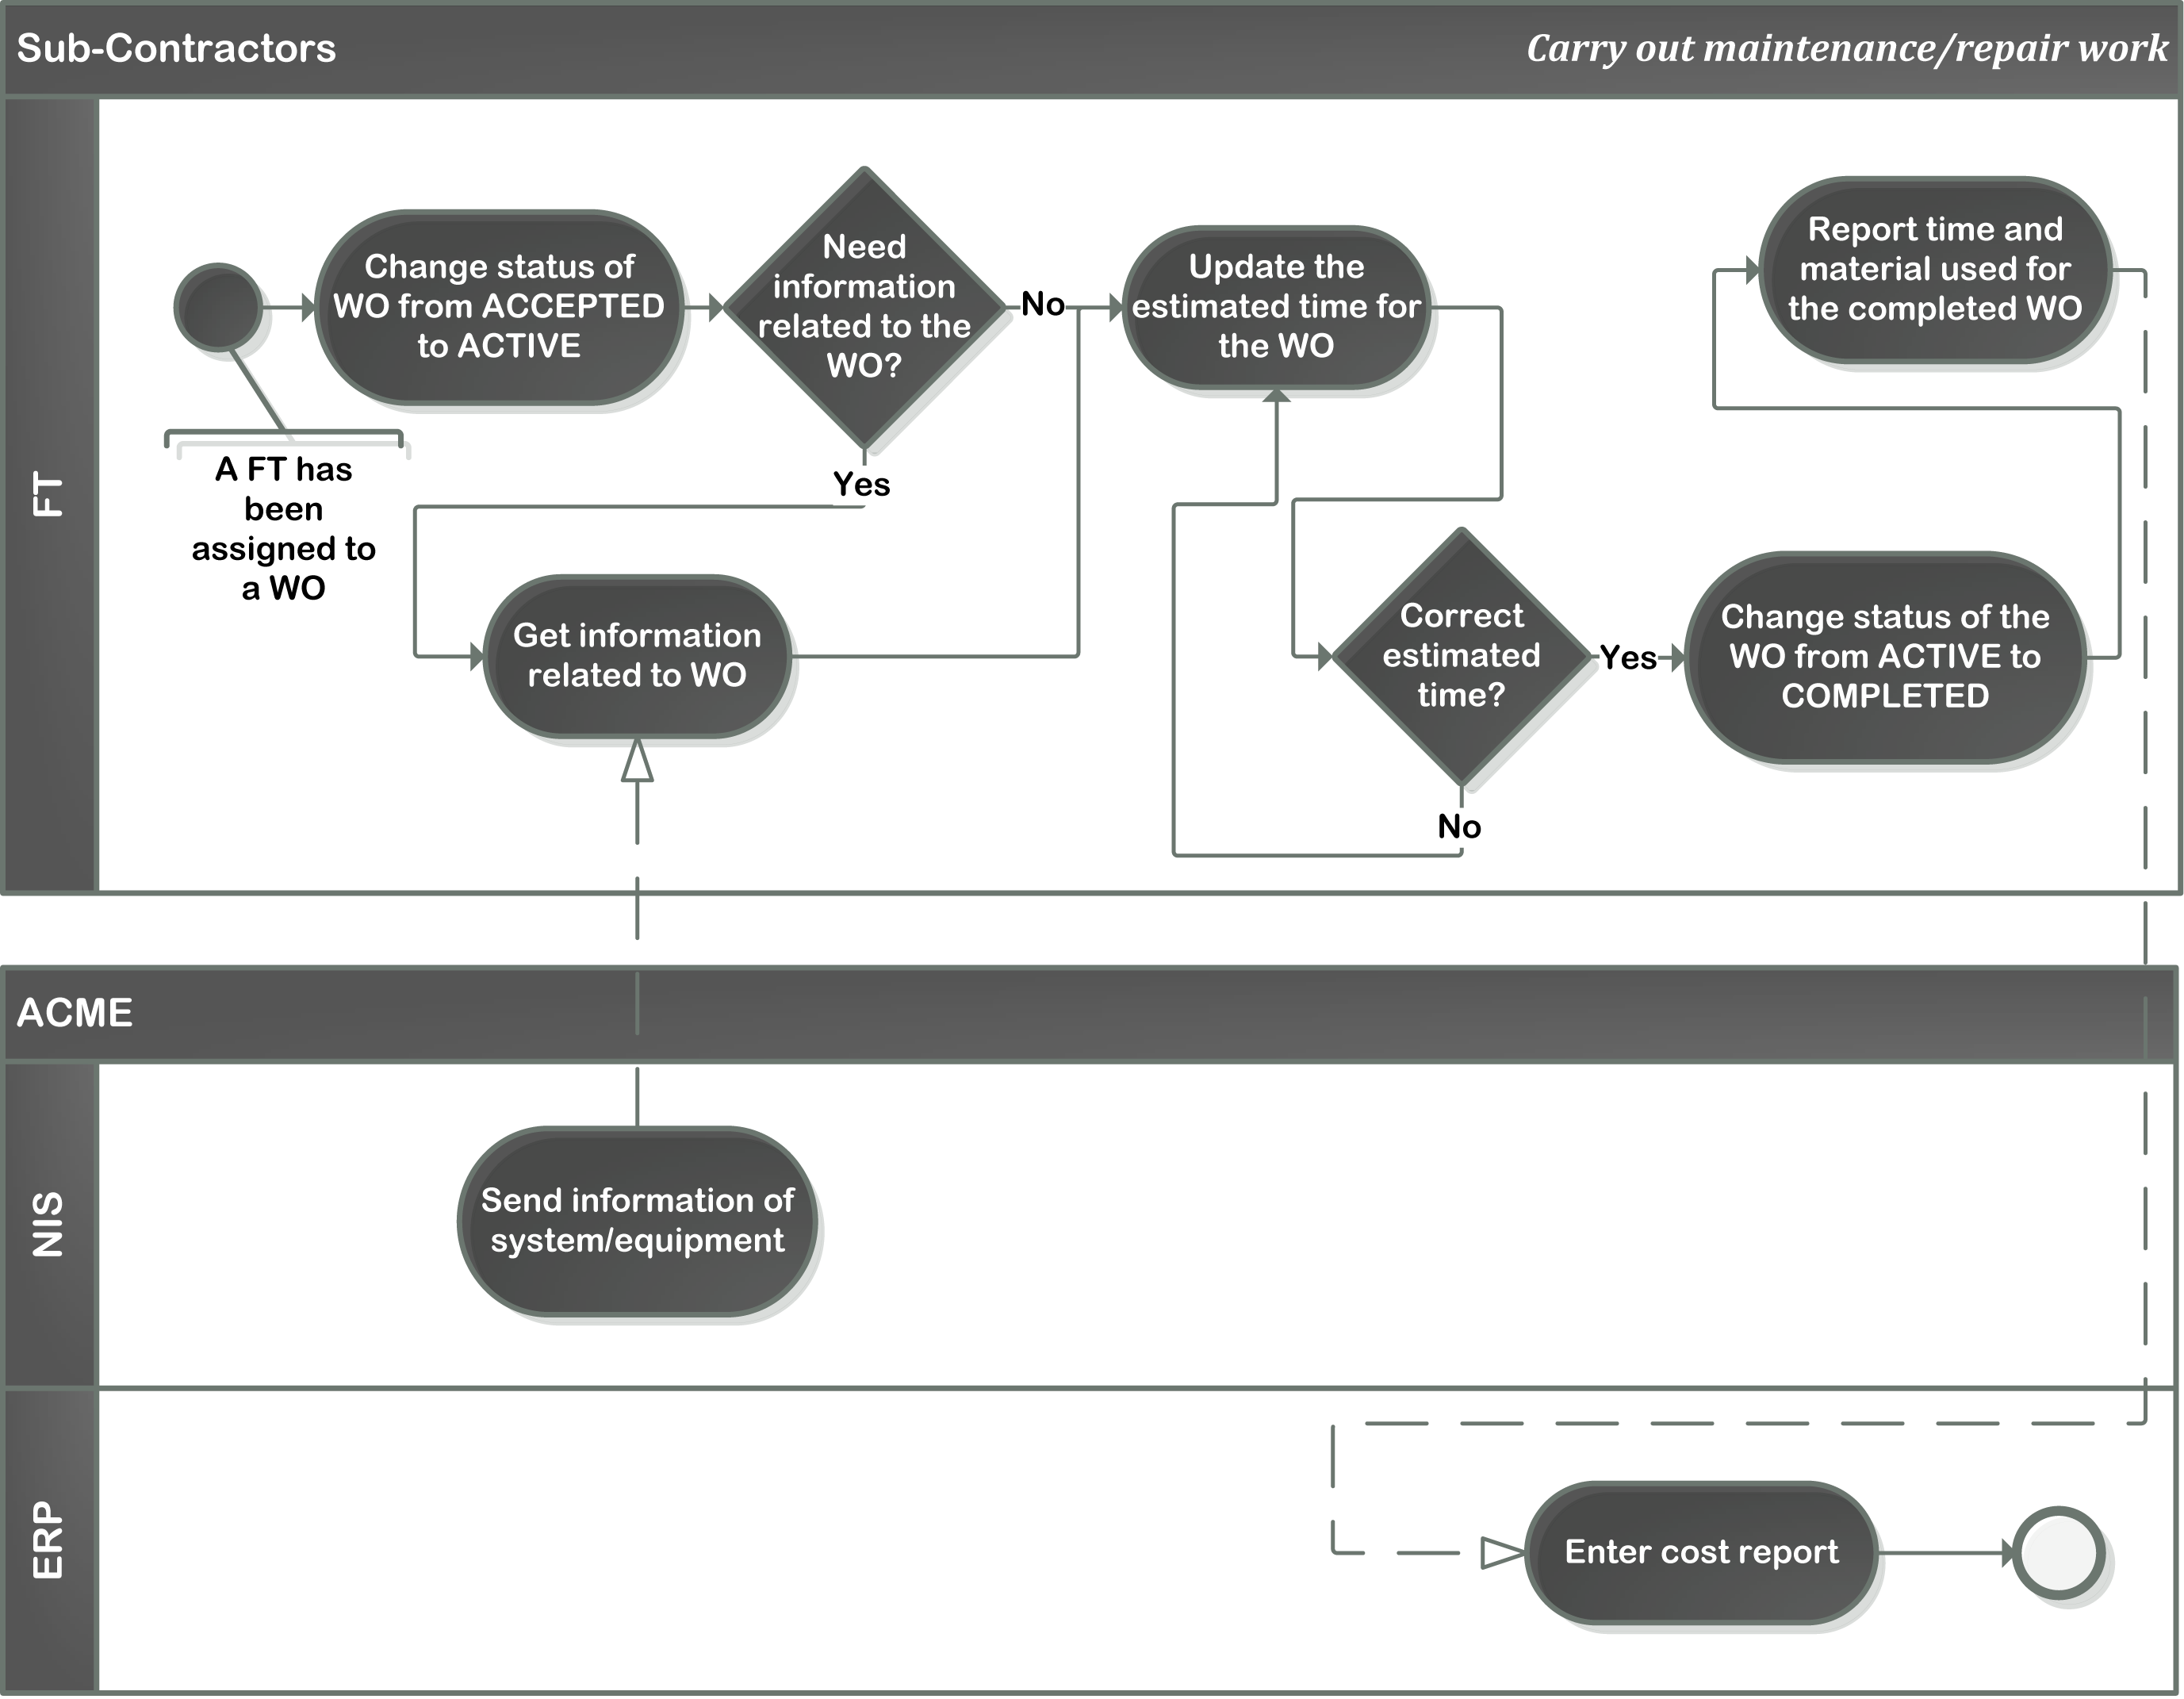
\includegraphics[scale = 0.7]{images/carry.png}}
	\label{fig:carry}
	\caption{Carry out maintenance/repair work}
\end{figure}
%
\subsubsection{Inform About Outages and Their Status}
\label{sec:bp5}
An important function in the ACME business is the relationship to their existing customers. Providing customer utility means not only deliver a good product, in this context $\rightarrow$ electrical power, but also nurtures the customer in terms of support. According to \emph{ACME Power Company - Appendix A} \cite{A}, \emph{''... the second largest share of calls concern outages.''}, hence the importance of this process, connected to GOALS-3 and GOALS-4, is of no doubt. 

Figure \ref{fig:inform} illustrates this process. Three stakeholders - M/E, MO, and FT - are providers of information concerning outages and their status. CC is the consumers of this information, and need to access it on customer demands. This data is located in the CIS.

The WOMS will support this system, as it will function as a man-in-the-middle system, with its purpose to greatly increase the quality of the outage information stored in CIS. As of today, this information is rarely completely updated \cite{A}, a fact WOMS will extinguish. WOMS shall continuously update this information in CIS and as described in \ref{sec:bp4}, where FTs could update this information in real-time, the status of an outage will always be up to date. 
\begin{figure}[H]
	\centering
	\setlength\fboxsep{7pt}
	\setlength\fboxrule{0.5pt}
	\fbox{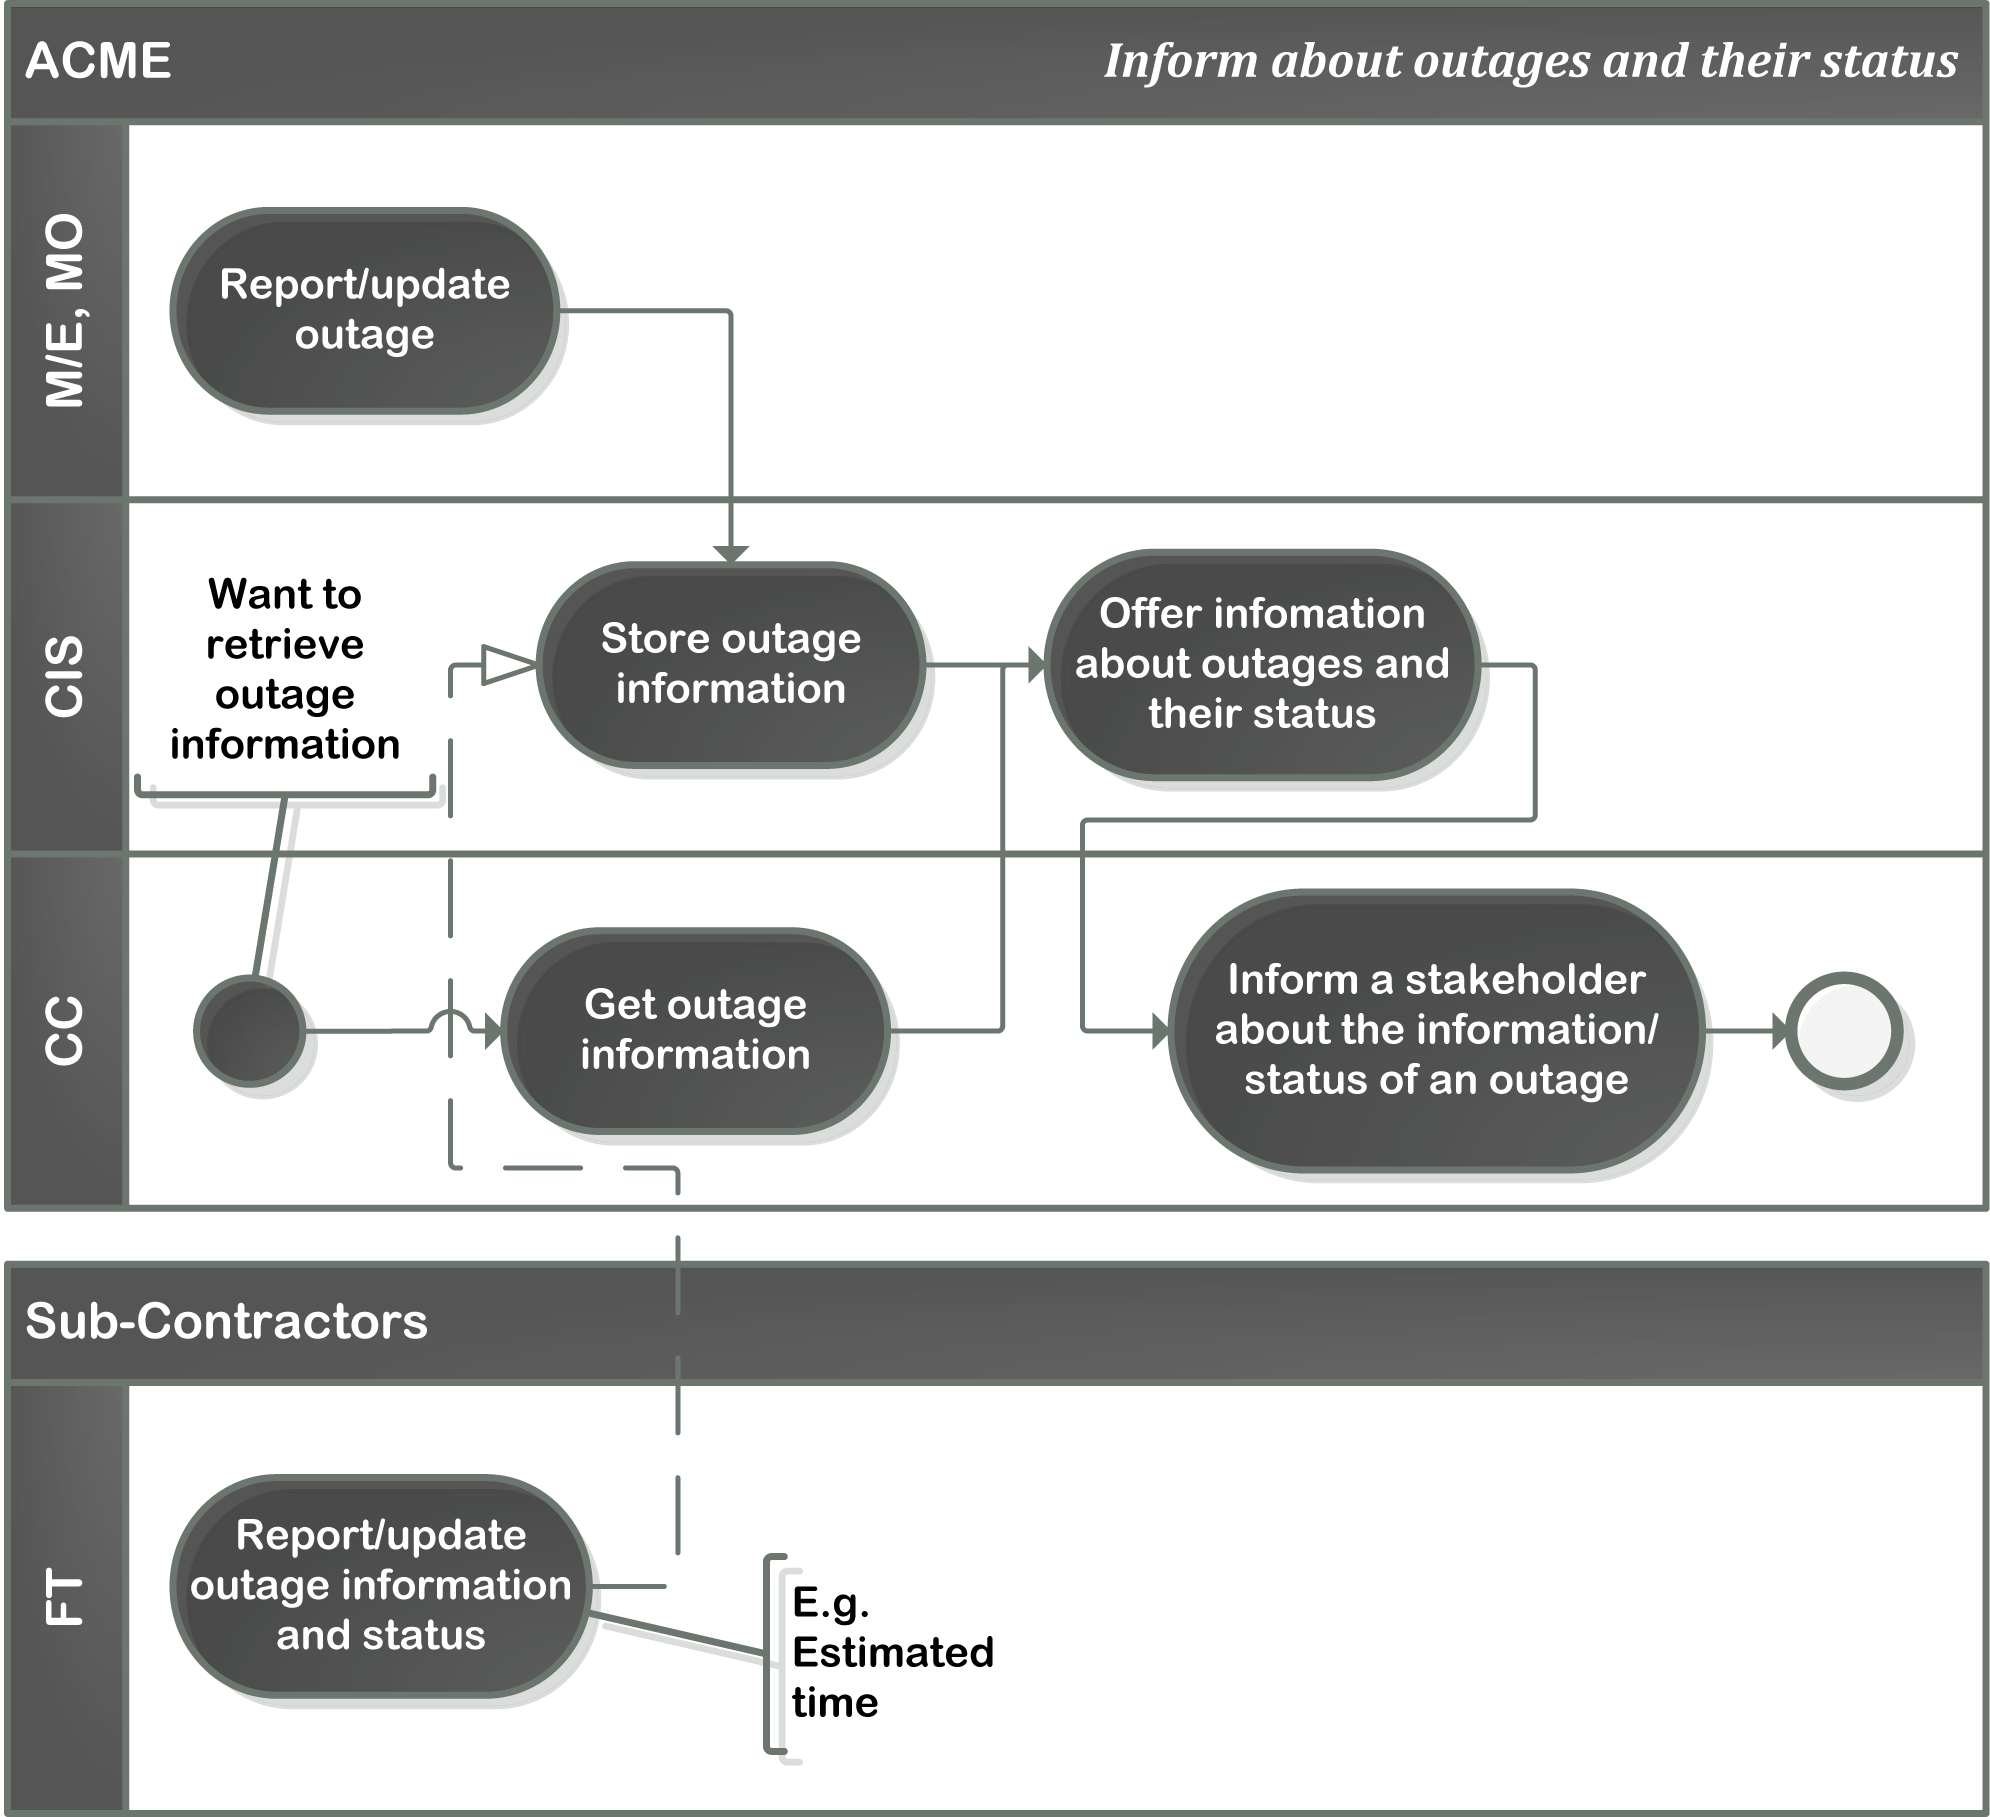
\includegraphics[scale = 0.7]{images/inform.png}}
	\label{fig:inform}
	\caption{Inform about outages and their status}
\end{figure}
%
\subsubsection{Analyze Cost and Repair Data}
\label{sec:bp6}
The process of analyzing costs and repair data consequently is a precondition to be able to come up with new solutions and improvement for routines and procedures. These are causes leading to fulfill GOAL-1 and GOAL-2. 

The stakeholder ACC begins gathering information concerning costs originating from maintenance/repair/\\construction work, e.g. differences in costs that different contractors (FTs) accounts for similar work orders/services.  Next step is to analyze the collected data, resulting in perhaps (to continue with the aforementioned example) valuable knowledge of which contractors that shall be hired in the future and which are not. 

WOMS supports this process by, simple, offer several types of statistics related to work orders. Such data is gathered by the system as we saw in process \ref{sec:bp4}. Today, this functionality is not provided by any system within ACME.
\begin{figure}[H]
	\centering
	\setlength\fboxsep{7pt}
	\setlength\fboxrule{0.5pt}
	\fbox{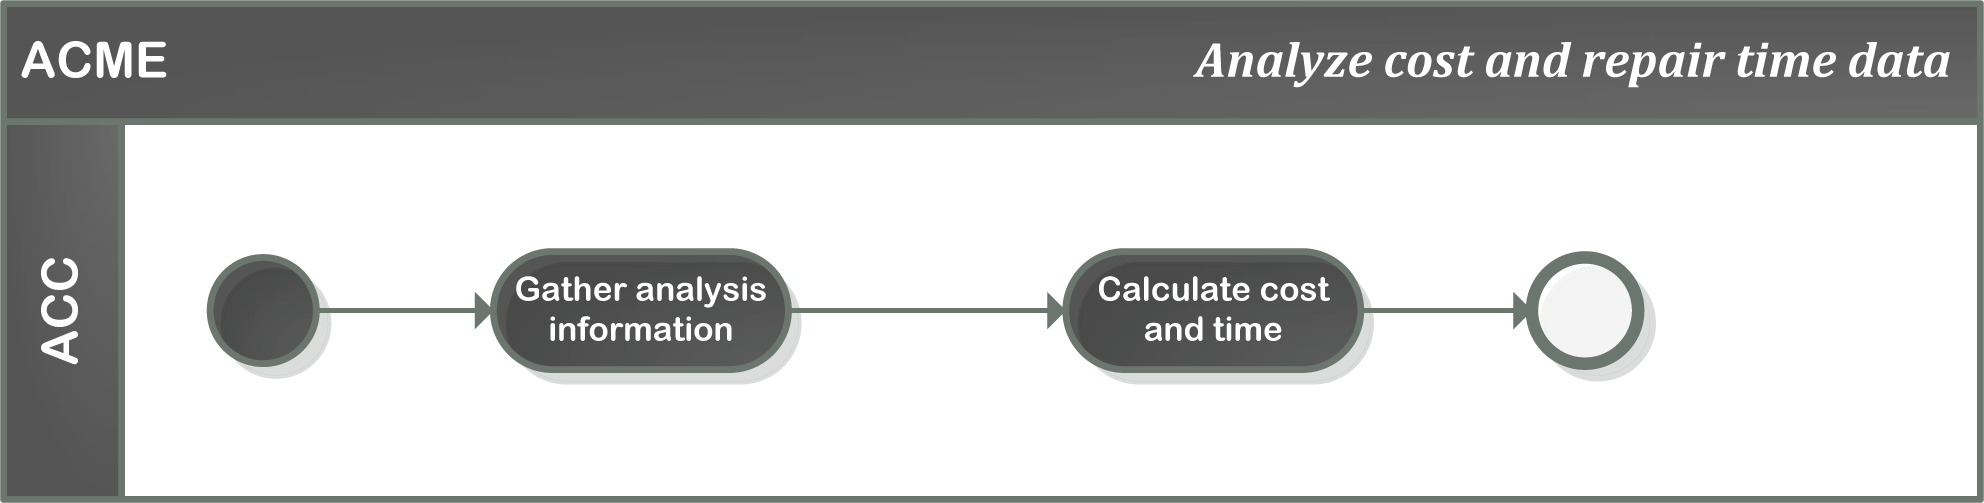
\includegraphics[scale = 0.7]{images/analyze.png}}
	\label{fig:analyze}
	\caption{Analyze cost and repair data}
\end{figure}
%
\subsection{Product Functions}

\subsection{Assumption and Dependencies}
\label{sec:assumption_and_dependencies}
The product WOMS specified in this document, with all of its requirements, is dependent on the ACME's current systems functionality. If, for example, there is no system like NIS where network equipment data is stored, WOMS will not be able to fulfill certain requirements - they depend of the functionality of a system like NIS. The same applies for other systems. 

To manage meeting GOAL-4, this procurement project is dependent on future project which we assume will be executed. The WOMS product itself will not be the reason this goal will be fulfilled. However, procuring and installing this WOMS will set preconditions for this change to take place.

\subsection{Design and Implementation Constraints}
\label{sec:desing_and_implementation_constraints}
In the table \ref{table:design_and_implementation_constraints}, design and implementation constraints affecting the implementation of WOMS are presented, extracted from \emph{ACME Power Company - Appendix A} \cite{A}.
\begin{center}
	\begin{longtable}{|l|p{5cm}|p{5cm}|}
		\caption{Design and implementation constraints}
		\label{table:design_and_implementation_constraints}\\
		\hline
		\textbf{ID} & \textbf{Constraint} & \textbf{Comment}\\
		\hline
		\endfirsthead

		\multicolumn{3}{c}%
		{\tablename\ \thetable\ -- \textit{Continued from previous page}} \\
		\hline
		\textbf{ID} & \textbf{Constraint} & \textbf{Comment}\\
		\hline
		\endhead

		\hline \multicolumn{3}{r}{\textit{Continued on next page}} \\
		\endfoot
		\hline
		\endlastfoot
		\hline
		2.6.1 & Apply open standards whenever possible & Concerns all ACME's system architecture \\
		\hline
		2.6.2 & Data flow from ACME computers to and from other networks shall pass through ACME's network boundary firewall proxy &
		See section \ref{sec:external_interface_requirements} for more information \\
		\hline
		2.6.3 & No modifications shall be done on the ERP system & WOMS must adapt to the ERP system \\ 
		\hline
	\end{longtable}
\end{center}